\documentclass[a4paper]{report}
% Package definition
\usepackage{graphicx}
\usepackage{setspace}
\usepackage{fancybox}

% added package
\usepackage[utf8]{inputenc}
\usepackage[cyr]{aeguill}
\usepackage{xspace}
\usepackage[english,french]{babel}
\usepackage{url}
\usepackage[nottoc,numbib]{tocbibind}
\usepackage{hyperref}
\usepackage{amsmath}
\usepackage{listings}
\usepackage{xcolor}
\usepackage{diagbox}
\usepackage{lscape}
\usepackage{tabularx}
\usepackage{geometry}


% hacks
\let\urlorig\url
\renewcommand{\url}[1]{%
   \begin{otherlanguage}{english}\urlorig{#1}\end{otherlanguage}%
}
% Default fixed font does not support bold face
\DeclareFixedFont{\ttb}{T1}{txtt}{bx}{n}{12} % for bold
\DeclareFixedFont{\ttm}{T1}{txtt}{m}{n}{12}  % for normal

% Custom colors
\usepackage{color}
\definecolor{deepblue}{rgb}{0,0,0.5}
\definecolor{deepred}{rgb}{0.6,0,0}
\definecolor{deepgreen}{rgb}{0,0.5,0}

% Python style for highlighting
\newcommand\pythonstyle{\lstset{
language=Python,
basicstyle=\ttm,
morekeywords={self},              % Add keywords here
keywordstyle=\ttb\color{deepblue},
emph={MyClass,__init__},          % Custom highlighting
emphstyle=\ttb\color{deepred},    % Custom highlighting style
stringstyle=\color{deepgreen},
frame=tb,                         % Any extra options here
showstringspaces=false
}}


% Python environment
\lstnewenvironment{python}[1][]
{
\pythonstyle
\lstset{#1}
}
{}

% Python for external files
\newcommand\pythonexternal[2][]{{
\pythonstyle
\lstinputlisting[#1]{#2}}}

%%%%%%%%%%%%%%%%%%%%%%%%%%%%%%%%%%%%%%%%%%%%%%%%%%%%%%%%%%%%%%%%%%%%%%%%%%%%%%%
%%%%% VARIABLE TO DEFINE %%%%%
\newcommand{\titreMemoire}{Génération de tests unitaires pour programmes Python}
\newcommand{\auteurMemoire}{Ortegat Pierre}
%%%%%%%%%%%%%%%%%%%%%%%%%%%%%%%

\makeindex

\begin{document}
\thispagestyle{empty}

\begin{center}
\textsc{Universit\'e de Namur}\\
Facult\'e d'informatique\\
Ann\'ee acad\'emique 2021--2022
\end{center}
\vspace{1.3cm}
\hspace{1.4cm}
\fbox{
\begin{minipage}[c][5.4cm]{9.6cm}
\large
\begin{spacing}{1.2}
\begin{center}
\textbf{\titreMemoire}\\
\vspace{1cm}
\auteurMemoire
\end{center}
\end{spacing}
\end{minipage}
}
\vspace{0.5cm}
\begin{figure}[!h]
~~~~~~~~\centering
\includegraphics[scale=4.0]{img/unamur.png}
\end{figure}

\normalsize

\vspace{0.5cm}
\begin{table}[!h]
\centering
  \begin{tabular}{ r l }
    Promoteur~: &  \rule{4cm}{0.1mm} {\small (Signature pour approbation du d\'ep\^ot - REE art. 40)}\\
    ~\underline& Xavier Devroey \\\\
    Co-promoteur~: & Benoît Vanderose\\
  \end{tabular}
\end{table}

\vspace{0.5cm}
\begin{center}
M\'emoire pr\'esent\'e en vue de l'obtention du grade de\\
Master en Sciences Informatiques.
\end{center}

\nocite{*}
\chapter*{Remerciements}

Je tiens à remercier mes promoteurs, Xavier Devroey et Benoît Vanderose pour leurs nombreux conseils avisés qui m'ont été donnés sans compter et plus particulièrement Xavier Devroey pour ses nombreuses relectures.
Elles en ont étonné plus d'un de par leur complétude et le temps minuscule qui se passait entre ma soumission pour relecture et le retour de bon conseils.

Je tiens également à remercier l'entreprise dont je fais actuellement partie, Oniryx, pour m'avoir soutenu dans cette aventure.


\chapter*{Résumé}

L'application de tests automatiques au code soumis par les étudiants sur une plateforme de correction automatique est un outil utile pour le corps enseignant.
Il permet de fournir de meilleurs retour, sur plus d'exercices, créés plus rapidement.
Des méthodes des tests automatiques sont analysées et une sélection est faite sur ceux qui, de par leurs caractéristiques, sont les plus intéressant dans le contexte de la correction automatique des codes d'étudiants.
Les méthodes retenues sont le fuzzing en boite grise et le test de combinaisons d'appels sur une structure donnée.
L'efficacité de celles-ci est discutée et une application pratique est développée sous la forme d'une librairie de test qui s'intègre dans la plateforme de correction automatique Inginious.
Les limitations sont analysées et un protocole de test des modifications apportées par celle-ci est ensuite proposé pour pouvoir quantifier les gains apportés via une expérience pratique.



\tableofcontents

\chapter{Introduction}

Les techniques de génération automatiques de tests permettent de fournir une aide utile au corps enseignant pour créer un retour rapide et pertinent sur les soumissions de code d'étudiants soumis dans le cadre d'un bachelier en informatique tout en permettant de ne devoir créer qu'un minimum de code lors de la mise ne place du cours et de ses exercices.

Le but de ce mémoire est d'évaluer les différentes techniques de tests automatique qui existent, de regarder dans quelle mesure elles sont adaptées à la correction de code d'étudiants dans le cadre d'une plateforme de correction automatique et d'évaluer l'apport effectué par cette technique à l'apprentissage des étudiants et au travail réalisé par le corps enseignant.

Pour ce faire, ce document est découpé en trois parties.

Dans un premier temps, un large éventail de technique de tests automatiques seront explorées; avec leurs défauts et avantages mis en avant.
Une sélection sera fait parmi celles-là.
Ensuite, une analyse sera faite de certains points pertinents à l'application desdites techniques de tests.
Enfin, un commentaire sera fait sur leur implémentation et un protocole de test pour vérifier l'efficacité de ce qui a été créé en pratique.

Une attention toute particulière à été gardée tout au long de l'analyse des techniques et de leurs conséquences pour que les résultats obtenus soient directement utilisables sur le terrain.
Pour ce faire un libraire de test automatique implémentant la sélection a été créé et intégrée à un runner Inginious.


\chapter{État de l'art}

%TODO sub-intro if deemed needed

\section{Méthodes de test}
Cet état de l'art couvre une série de méthode de test de composant logiciels, qu'il soient auto-contenus ou distribués.
Tous ceux listés dans cet état de l'art ont été considérés pour être intégrés dans le travail décris après.
Ils n'ont été tous intégrés pour des raisons décrites plus loin.


\subsection{Tests manuels}

%Le style le plus classique et ancien
Pour des raisons de complétude, il est intéressant d’inclure dans cette liste de méthodes et techniques de test la façon la plus ancienne qui existe: l’écriture et l’utilisation de tests unitaires.
Ces tests, bien que plus ciblés et directs que les tests automatiques ne sont pas sans défauts.

% Prends du temp
Ils sont plus lents à écrire et nécessitent beaucoup plus de ressources que leurs contreparties automatiques.
%pas tjrs adapté / bien fait \& parfois ne couvrent pas le code / les features correctement \cite{Zhu1997} 
De par la nature humaine de leur création, ils ne seront pas toujours adaptés, bien conçus ou n'auront pas une bonne couverture du code et des fonctionnalités mais pourront être plus concis dans le cas de test précis \cite{Zhu1997}.

%biais de confirmation \cite{Calikli2014} => solution bdd
Un autre problème récurrent rencontré lors de l'utilisation de tests unitaires écrits à la main est un problème de biais de confirmation.
En effet, il n'est pas rare d'observer que les tests unitaires écrits soient juste une confirmation de ce que le développeur a écrit et non ce qui a été demandé comme fonctionnalité \cite{Calikli2014}.
Ce biais de confirmation rend l'utilisation de ces tests unitaire inutile car la seule chose qu'ils vont confirmer est que l'implémentation du développeur initial est bien celle utilisée.
Une méthode utilisée pour combattre ce phénomène est de faire du développement par le comportement (appelée BDD = Behavior Drive Developpement dans l'industrie) qui va consister à écrire les tests avant d'écrire le code et, idéalement, que ces tests initiaux soient écrits par quelqu'un d'autre que le développeur de la fonctionnalité.

%flackiness \cite{Luo2014}
Un autre problème classique récurent des tests unitaires écrits à la main est la “flackiness” (i.e. l'instabilité d'un test lorsque que celui-ci est exécuté plusieurs fois).
Ce problème diminue fortement l'efficacité des-dits tests, car ils ne permettent plus de s'appuyer dessus afin de garantir que le software fonctionne correctement.
Des erreurs de tests à la fréquence assimilable à de l'aléatoire, n'apportent aucune information pertinente supplémentaire \cite{Luo2014}.


%=> techniques automatiques utiles, cqfd
Ces divers problèmes et défauts des tests unitaires écrits à la main ont mené au développement d’autres techniques, dont le fuzzing, qui va être décrit dans la section suivante.

\subsection{Fuzzing}

Lors de son invention, le terme “Fuzzing” avait pour signification de fournir rapidement et en grand nombre des entrées aléatoires à un programme, dans le but d'en augmenter la robustesse \cite{Forrester2000}.

Aujourd’hui, les pratiques regroupées sous le terme fuzzing sont nombreuses et variées et servent plusieurs buts différents.
L'utilisation la plus classique  de cette technique est la sécurisation des parties de logicielle qui interagissent avec des entrées extérieures \cite{Godefroid2020} (on peut par exemple citer le fait que du fuzzing est une des étapes incluses dans le "Microsoft Security Development Lifecycle" \cite{howard2006security} ).
Avoir fuzzé une interface logicielle ne garantit pas que cette interface est sans faille ni bugs mais permet de raisonnablement considérer que l'interface est sécurisée et sans bugs\cite{Godefroid2020}.


%Ajdh: fort utilisé dans la sécu dès qu'il y a un user input \cite{Godefroid2020} (fait partie du Microsoft Security Development Lifecycle \cite{howard2006security})

\subsubsection{Fuzzing en boite noire}

%Prendre tt le prob et donner à l'aveugle des inputs \cite{Forrester2000}
Le fuzzing dit “en boite noire” est une des approches possile du fuzzing.
Elle va considérer trois éléments lors de chaque test:
\begin{itemize}
\item Les entrées fournies au programme
\item Les réponses données par le programme (\textit{toutes} les sorties et effets de bord du programme sont pris en compte; cela inclus les erreurs)
\item Le programme en lui-même qui va être considéré comme une unité atomique, aucune observation ne sera faite sur l'état interne du programme.
\end{itemize}
Des entrées vont être générées à l'aveugle, fournies au programme et le résultat va être enregistré \cite{Forrester2000}.
Si le résultat n'est pas satisfaisant, les entrées qui ont déclenché ce résultat vont être conservées et remontées pour qu'une correction puisse être effectuée.

%Dépend critiquement d'un set de seed valides à la base si on veut être efficace
Le principal  défaut de cette méthode de test est qu'elle est fortement dépendante de la qualité des entrées initialement fournies ou générées. 

Par exemple: le cas d'un programme très simple qui ne prend qu'un paquet Ethernet en entrée.
Le contenu maximum d'une trame Ethernet est de 1500 bytes (pour l'exemple, on considère que la trame Ethernet est elle-même bien formée).
Pour couvrir l'intégralité des probabilités d'entrée du programme, il est nécessaire de générer et de tester le nombre suivant de possibilités:

$$2^{1500 * 8} \approx 2,2905 * 10^{3612}$$

Sachant que le microprocesseur le plus rapide de tous les temps, d'après le Guiness World Record, est de $8,42938$ GHz\cite{gwrcpu}, si l'on teste une possibilité par avancée d'horloge du microprocesseur, il faudra $\frac{2^{1500*8}}{ 8429380000}$ secondes pour tester complètement ce programme
$$\approx 8,6167 * 10^{3594} \text{ années}$$

ce qui est, en pratique, infaisable et souligne l'importance d'avoir des entrées initiales pertinentes.
Au travers de cet exemple, il est clair que le fuzzing en boite noire ne peut pas espérer tomber au hasard sur tous les cas problématiques, il doit avoir des entrées déjà proches de ce qui pourrait causer des bugs.


%important aussi de limiter le bruit inutile et pas générer plein de shizer
Les entrées initiales, en plus d'être bien formée au début, doivent être modifiées de façon intelligente par rapport au problème.
Soumettre à répétition des entrées complètement fausses ne servirait à rien: le programme le détectera et les ignorera rapidement ; ne testant que peu de possibilités d'exécution \cite{Godefroid2020}.

\subsubsection{Fuzzing grammatical et en boite grise}

%greybox fuzzer: \cite{fuzzingbook2022:GreyboxFuzzer}
Le fuzzing en boite grise (aussi appelé fuzzing en "greybox") est la même pratique que de le fuzzing en blackbox, à une différence près.
Dans ce cas-ci, on va se servir d’indications puisées directement dans le programme testé pour orienter la recherche \cite{fuzzingbook2022:GreyboxFuzzer}.

Dans le cas de Python, une des approches possible est de compter le nombre de lignes de codes qui ont été exécutées avec une entrée donnée.
Plus une entrée a permis à un grand nombre de lignes d’être exécutés, plus celle-ci va être réutilisée et mutée rapidement.
Les entrées quoi n'atteignent presque aucunes lignes verront leur utilisation être nettement diminué \cite{fuzzingbook2022:GreyboxFuzzer}.

%greybox grammar fuzzer: \cite{fuzzingbook2022:GreyboxGrammarFuzzer}
\paragraph{Le fuzzer en boite grise à grammaire} ajoute l'utilisation d'une grammaire pour former des entrées qui seront valides et, ainsi, explorer l'espace des entrées possibles plus efficacement en ignorant celles qui seront rejetées rapidement \cite{fuzzingbook2022:GreyboxGrammarFuzzer}.
Le défaut de cette approche est qu'elle ne teste que des entrées qui sont valides.
La combiner avec une forme de mutation d'entrées est, dans beaucoup de cas, intéressant et permettra d'avoir de meilleurs résultats.

Parmis les outils de fuzzing en boite grise classique, on peut notamment citer \cite{sutton2007fuzzing}:
\begin{itemize}
\item Peach (qui est intégré dans Gitlab a présent) \cite{peach}
\item Spike \cite{spike}
\item Sulley \cite{sulley}
\end{itemize}

%g fuzzing pour trouver des failles de sécu dans les browser:  \cite{holler2012fuzzing}

%g fuzzing trouver bug complexes dans des compilateurs C  \cite{yang2011finding}

%g fuzzing pour trouver les bugs dans les proto réseaux \cite{aflnet}

Ce type d'approche est utilisé dans plusieurs applications pratiques, tel que la recherche de failles de sécurité dans les navigateurs \cite{holler2012fuzzing}, la recherche de failles de sécurité dans les compilateurs C \cite{yang2011finding}, la recherche de bug dans les implémentations de protocoles réseaux \cite{aflnet}.


%apprentissage auto gramaire : \cite{bastani2017synthesizing}
%tracer process pour créer gramaire automatiquement \cite{hoschele2017mining}
Il est possible de designer un fuzzer qui apprendra automatiquement sa grammaire via divers moyens, tel que le tracing d'exécution \cite{hoschele2017mining} mais ils ont un intérêt limité car il y a un risque, non-négligeable, que la grammaire apprise inclue les erreurs du programme.
Cela ne sera pas systématiquement le cas mais faire attention à ce problème est nécessaire lors du design d'un système de fuzzing (pour y remédier une approche en portfolio peut être utilisée).

%limité par la grammaire en elle même, plus gros défaut
La limitation majeure de l'utilisation d'une grammaire pour générer des entrées valides est la grammaire en elle même.
De par sa nature, elle est limitée à des entrées bien formées et ne peut pas tester les cas limites qui sont faux mais très proches d'un cas correct.
Une autre limitation de cette technique héritée de la façon de fuzzer en boite noire est sa dépendance à un set d'entrées initiales.
Si elles ne sont pas représentatives et exhaustives des cas intéressants ou problématiques, le fuzzer n'aura que très peu de chance de trouver les cas problématiques.

\subsubsection{Fuzzing en boite blanche}

%parser le prog, le faire tourner et tenter de résoudre les conditions pour toucher toutes les branches avec un solveur.
Le fuzzing dit "en boite blanche" est une variante de fuzzing plus informée.
Celle-ci va commencer comme du fuzzing en boite noire mais va, au fur et la mesure de l'exécution, récolter des information et condition nécessaire pour atteindre plus de branches d'exécution (idéalement toutes mais ce n'est pas toujours possible).
Les conditions récoltées lors d'une exécution seront résolues par un solveur logique et les nouvelles entrées crées par cette résolution vont être utilisées pour les prochaines exécutions du code testé.
Ce mélange d'exécution concrète et symbolique (via la résolution de contraintes) a donné le nom de "testing concolique" à cette méthode de test.
%Plus efficace pour un covering complet et pour taper sur toutes les branches et chopper les bugs de meeeeeeeeeeeeeeeeeeeeeeeeeeeeeeeeeeeeeeeee
Elle est particulièrement efficace pour aller chercher les cas particuliers et atteindre une couverture de code particulièrement élevée.

%dynamic execution testing: SAGE \cite{godefroid2008automated} (symbolic execution x86 level avec opti pour enorme stack traces \cite{Godefroid2020} ) 
Un exemple pratique de l'application de cette méthode est l'outil SAGE actuellement développé et maintenu par Microsoft\cite{godefroid2008automated}.
Sage est un fuzzer qui teste en faisant de l'exécution symbolique x86 en boite blanche qui est optimisé pour gérer des stack trace énormes\cite{Godefroid2020}.

Cet outil est utilisé dans une des étapes finales de release des produits Microsoft et, régulièrement, découvre ce  qui est appelé un "bug à millions".
Les bugs à millions sont des bugs qui, s’ils passent en production, couteraient collectivement, aux utilisateurs finaux, plus d'un million pour résoudre, patcher et re-déployer le code problématique \cite{Godefroid2012}.

%qui étend le travail d'autre sur la génération de tests auto \cite{Godefroid2020} \cite{cadar2005execution} \cite{godefroid2005dart}
SAGE étends d'autres travaux déjà réalisés dans le domaine de l'exécution concolique automatique \cite{Godefroid2020} \cite{cadar2005execution} \cite{godefroid2005dart}.
Cet outil n'est pas qu'un outil utilisé en recherche académique et a, actuellement, des utilisations dans l'industrie.
Sa principale utilisation est faite par Microsoft, notamment pour le débug des OS depuis Windows 7.
%utilisé en prod partout, plus de 100 années machines dans les dents
Il est estimé que depuis sa mise en service en 2008, il a fuzzé des centaines d'applications Microsoft en continu sur des centaines de machines et que SAGE a déjà accumulé plus de 100 années-machines d'exécution\cite{Godefroid2012}.

%"largest computational usage ever for any Satisfiability-Modulo-Theories (SMT) solver" d'après les auteurs de z3 \cite{moura2008z3}
Les auteurs du solveur logique Z3 ont qualifié l'utilisation de Z3 par SAGE de la façon suivante:
\begin{center}
"Largest computational usage ever for any Satisfiability-Modulo-Theories (SMT) solver" \cite{moura2008z3}\\
\begin{center}
\line(1,0){2.5cm}$ $ \\
\end{center}
L'utilisation la plus grande de tous les temps d'un résolveur SMT [trad] 
\end{center}

\subsection{Property based testing}

Le test par propriété est une variante, plus poussée, du fuzzing décrit avant.
En effet, c'est une forme de fuzzing mais les différentes entrées vont être générées à partir des propriétés qui sont définies pour chaque entrée.
Initialement développé en et pour Haskell, l'utilité d'une telle forme de test, surtout dans les programmes définis strictement ou par contraintes mathématiques, s'est avérée grande \cite{Paraskevopoulou2015}.

Ces propriétés définie sur les entrées vont être données à un oracle qui va les traduire en entrées valides pour le programme, d'après leur définition.
Ces entrées vont pourvoir être ensuite testées avec le programme en question afin de vérifier que celui-ci ne présente pas de comportement non-désirable \cite{Fink1997}.
Un autre oracle peut être définit pour contraindre quelles sont les états finaux valides ou non.

L'avantage d'utiliser un tel système est qu'il est possible de couvrir tous les cas particuliers connus liés aux propriétés d'entrée plus facilement.
En effet, avec les contraintes définies sur les entrées, il est possible de définir une série d'entrées liées à celles-ci.
Un autre avantage est qu'une fois une entrée problématique a été trouvée, il est possible d'utiliser l'oracle pour réduire cette entrée à une définition minimum afin d'aider au débug du code sous-jacent \cite{Papadakis2011}.

Cette méthode présente deux défauts majeurs.

Le premier est qu'elle ne permet pas, comme le fuzzing, de garantir que le programme donné est juste.
Elle permet uniquement d'assurer qu'il l'est partiellement (avec les entées testées, d'où la nécessite de faire de tests exhaustifs) \cite{Papadakis2011}.

Le second est que le set de contraintes / propriétés à écrire pour les entrées est long a définir et peut, dans certains cas, revenir  a réécrire une partie du programme lui même.
Cela, dans le cas où les propriétés sont définies assez précisément pour qu'elles soient utiles \cite{Papadakis2011}.

\subsection{Injection de fautes}

L'injection de fautes est une méthode de test consistant à injecter des erreurs dans le programme testé.
Il existe deux façons principales de le faire.


\paragraph{Introduire des erreurs au niveau hardware} est une méthode qui est très peu utilisée à l'échelle du développement logiciel non dédié à du matériel spécialisé.
Cette méthode consiste à, directement au niveau du matériel, provoquer des erreurs (changement de bit temporaire ou non, erreur d'accès aux diverses parties du matériel, erreurs réseaux…)\cite{Avresky1996}.

\paragraph{Introduire des erreurs au niveau logiciel} est la façon la plus répandue de faire des tests par injection de fautes.
Il est possible d'en faire à divers niveaux, en boite noire et en en boite blanche.
Cette méthode teste principalement la robustesse du code testé et sa capacité à récupérer des erreurs.
Une autre utilisation, est de tester si des tests unitaires sont à même de détecter des bugs (cette technique est aussi appelée du test par mutation).

Pour utiliser l'injection de faute pour tester les tests unitaires, une ou plusieurs fautes seront injectées dans le code.
Le test réussira si les tests unitaires détectent et échouent à cause de l'erreur injectée \cite{Segall}.

Le test de gestion d'erreurs et de robustesse sert à vérifier que la gestion d'erreurs est correcte, que le code / le composant testé sait récupérer correctement d'un problème et de prévoir la façon dont certaines fautes vont de dérouler \cite{Avresky1996} (on peut appliquer cette méthode à des systèmes entiers \cite{Lenka2018}).
Ils serviront également à déterminer la "zone d'éclat d'une erreur": a quel point celle-ci va avoir un effet profond et grand sur le reste du composant testé.
Ces tests sont particulièrement utiles pour simuler les erreurs difficiles à simuler en tests unitaires ou bien qui demandent d'émuler un système d'exploitation complet \cite{Marinescu2011}.

Ces erreurs peuvent être injectées à plusieurs endroits différents; Dont le code source initial, le binaire une fois compilé, la mémoire durant l'exécution ou encore, à un niveau plus macro, supprimer/modifier/corrompre une instance d'un déploiement distribué \cite{Avresky1996}.

\subsection{Utilisation conjointe}

%NOTE: all can be combined to try to be more efficient !! \cite{Godefroid2020} => Hybrid fuzzing
Toutes les techniques de fuzzing décrites précédemment peuvent être combinées pour arriver à un résultat plus efficace que leurs performances individuelles \cite{Godefroid2020}.
Cette approche s'appelle faire du fuzzing hybride et est utilisée pour minimiser les problèmes liés aux différentes techniques. 


% plusieurs approches en meme temps: Portfolio approaches.
Dans le cas d'une approche encore plus générale, on parlera plutôt d'une approche en portefolio \cite{Godefroid2020}.
Comme le fuzzing hybride, le but est de minimiser les problèmes de limitations de chaque technique tout en exploitants leurs points forts.

\section{Tests unitaires \& éducation}

En 2012, suite à la constatation qu'il manquait des professeurs d'informatique, spécialement pour les 12-18 ans, l'outil Pythia a été créé.
Cet outil vise à complètement enlever le professeur de la boucle de feedback tout en permettant à l'étudiant de progresser. Il inscrit dans la philosophie d'apprendre en faisant qui s'avère être très répandue au développeur de cette tranche d'âge \cite{combefis2012teaching}.

L'université Catholique de Louvain a adopté cette plateforme et a ensuite, afin d'en dépasser les limitations, a créé une nouvelle plateforme appelée Inginious (d'autres universités ont également créé leur propre plateforme, par exemple L'Université Nationale de Colombie avec UNCODE \cite{restrepo2018uncode}).

Inginious est une plateforme FOSS (Free Open Source Software - Un logiciel gratuit et open source) web de gradation automatique de soumission étudiant.
Le code des étudiants va être compilé et exécuté dans un environnement sécurisé et, si celui-ci est correct l'utilisateur en sera informé.
Le cas échéant, une information pertinente lui sera fournie.

Pour illustrer les développements qui ont actuellement lieu dans la correction automatique des étudiants et en raison de l'abondance de littérature à son sujet, la plateforme Inginious va être prise comme référence.

Cette plateforme est l'objet de nombreux développements actuellement qui ont pour but de répondre à divers challenge apparu récemment.
L'un d'entre eux a été de fournir un feedback plus rapide et plus personnalisé à chaque étudiant, peu importe la quantité dont il a besoin\cite{Staubitz2017}.

Cette plateforme a également été utilisée pour répondre au besoin de correction des participants à un MOOC et permet à tous les étudiants d'avoir une correction adaptée et d'être certains de où ils se situent dans leur apprentissage\cite{derval2015automatic}.

Elle a été adaptée pour tous types de cours, pas seulement les cours de programmation.
Les cours de réseaux (et les exercices complexes liés à celui-ci) sont également intégré dans cette plateforme \cite{Bonaventure2020}.

Elle a également été adaptée pour les enfants, revenant ainsi sur les pas de son prédécesseur tout en apportant son lot d'améliorations \cite{Thuin} dont, entre autres, l'intégration de blocks "Blocky" (une forme de développement visuel).

Parmi les améliorations récentes de ce mode d'apprentissage, on peut notamment citer l'intégration de labels afin de donner un feedback plus précis \cite{Martin}, l'amélioration desdits feedbacks pour être plus pertinents et avoir plus d'impact \cite{Derval2022}, ...

Cette plateforme apporte également des nouvelles opportunités au corps enseignant de connaitre le niveau des étudiants avant l'évaluation.
Une variante avancée de cette pratique est l'utilisation d'intelligence artificielle pour déterminer à l'avance si un étudiant va réussir l'évaluation finale du cours \cite{Hormaux}.

% =====================================================================

\chapter{Problématique}

% descriptiuon du problème et du but
Dans le cadre de la création de nouveaux cours de programmation et d'algorithmique, le corps enseignant de l’Unamur a envisagé d'utiliser la plateforme d'apprentissage Inginious comme support de développement \& correction.
L'utilisation de cette plateforme implique la création de nombreux tests unitaires afin de fournir un feedback pertinent, rapide et approprié aux étudiants.
La taille et la complexité de cette tâche a poussé à la création de la question de recherche suivante;
\begin{quote}
Dans quelle mesure les techniques de génération automatique de tests permettent elles de fournir un retour aux étudiants dans le cadre d'exercices de programmation en bachelier informatique ?
\end{quote}
%Y a t il moyen d'automatiser, au moins partiellement ces tests ?
%Tout grain de temps pertinent, du point de vue enseignant comme du point de vue étudiant est considéré comme intéressant à creuser.

Suite à la réunion de kikoff, il a été déterminé que ce travail se concentrera sur les applications automatiques de tests unitaires suivants diverses stratégies.
Il a été déterminé que toutes les stratégies de tests classiques seront évaluées.
Les plus pertinentes seront implémentées et intégrées dans la plateforme Inginious.
Une attention toute particulière doit être apportée à la simplicité d’utilisation (le but principal de ce travail est de gagner du temps) et la qualité du feedback fourni aux étudiants.
 
 
\section{Sélection de stratégie de tests}

% pourquoi est ce que les tests sélectionnées ont été sélectionés
Parmi tous les types de tests considérés, certains n'ont pas été retenus.
Cette section va décrire pourquoi ils ont été écartés.
Des innovations ont été ajoutées pour mieux détecter certains problèmes moins soulevés par les autres stratégies dans le code testé.

Un facteur qui  a été pris en compte pour la sélection des stratégies de tests a été la limite de temps.
En effet, le temps de développement de ce projet n'étant pas illimité, les stratégies de tests trop complexes à mettre en place pour un retour moindre n'ont pas été retenues.

Parmi les stratégies non implémentées, il y a les tests concoliques (= une forme de fuzzing en boite blanches) qui demandent une intégration complète dans le solutionneur logique Z3 et une instrumentation complète de tout l'interpréteur Python.
Il a été estimé plus sage de se concentrer sur toutes les autres techniques afin de maximiser les résultats du projet au lieu de se concentrer sur celle-là.

Dans le reste de cette section, nous revenons sur les différentes approches et discutons leur inclusion ou exclusion de la liste des techniques adoptées.


\subsection{Tests par propriétés}

%nope, trop compliqué à correctement / complètement définir pour des tests rapides par rapport à du fuzzing.
Les tests par propriétés sont très intéressants dans le cas d'application définie très précisément qui ont besoin d'un haut niveau de fiabilité.
Ce n'est pas l'approche prise par ce mémoire-ci, qui vise plutôt à pouvoir créer rapidement des tests avec une quantité de code et de définitions d'entrées limité.
Écrire des définitions complète diminuerait fortement l'objectif d'écrire un minimum de code à l'impact de correction le plus grand possible.

Écrire des propriétés d'entrées vagues ou imprécises pour gagner du temps ou en généricité ne feraient que rabaisser l'efficacité et l'approche de cette méthode test à un équivalent au fuzzing en boite noire.
Cette technique étant considérée à part, il ne reste plus d'intérêt à faire des tests par propriété. 

\subsection{Injection de fautes}

%pas pertinent: on teste pas des tests unitaires, on ne teste pas le niveau de récupération et partillement rendondant avec l'apporche par seed a couverture du fuzzing
Les tests par injection de fautes sont principalement utilisés dans deux cas: le test de la qualité de tests unitaires et le test du code de récupération en cas d'erreur.

Le test de la qualité des tests unitaires n'est pas intéressant dans ce cas-ci: ils sont générés à la volée et s'adaptent dynamiquement au problème posé ce qui rend la génération de tests par injection de fautes impossible dans une majorité des cas.
Les cas restant sont des cas qui ne feront que confirmer ce qui a été explicitement mis en avant ou détecté par le code de génération de tests.

Le test de code de récupération est déjà ce que l'on va tester lors du fuzzing en essayant un maximum d'atteindre toutes les branches du code, dont celles de récupération.
Si un cas n'est pas proprement récupéré alors que c'est demandé dans le cadre de l'exercice, cela sera repéré et remonté avec la comparaison du code testé au code de référence.
En effet, le fuzzer qui a été développé compare le code testé à un code de référence et remonte une erreur si les sorties des actions ou les erreurs levées ne sont pas les mêmes.

\subsection{Fuzzing}

%intro fuzzing: kékécé ?
Durant la création de la librairie de test, certaines formes de fuzzing ont été fortement utilisées.
Le fuzzing a été sélectionné dans ce cas-ci, car cette technique permet de découvrir un maximum de problèmes relativement rapidement, peu importe le code testé.
Cette section va couvrir différentes techniques de fuzzing, leur avantages et leurs défauts et quelles décisions ont été prises quant à l'utilisation de celles-ci.


\subsubsection{Fuzzing en boite noire}

%nope redondant avec grise qui va faire mieux
Le fuzzing dit "en boîte noire" ou "à l'aveugle" est un technique qui est intéressante d'appliquer quand le système testeur / de fuzzing a déjà un indice sur le type d'entrée qui pourraient être pertinentes ou qui pourraient causer des problèmes.
Dans le cas de ce projet-ci, comme le code se veut très flexible et qu'il doit d'adapter à tous les exercices qui peuvent lui être soumis, cette approche n'est pas très réaliste si l'on veut être efficace et trouver les problèmes existants avec le code.
L'approche du fuzzing en boite noire n'a donc pas été sélectionnée dû à son manque de flexibilité si l'on désire obtenir des résultats pertinents rapidement.

\subsubsection{Fuzzing en boite blanche}

%nope no time + too complex for here + z3 is a piece of crap when used with Python
Le fuzzing en boite blanche et ses techniques associées (comme les tests concoliques) a été sérieusement considéré mais n'a pas été sélectionné par manque de temps et un problème de dépendance de version.
Cette section couvre les raisons de cette décision.


Le principal problème qui a complexifié énormément l'intégration de tests en boite blanche est la dépendance énorme que ceux-ci vont avoir sur la version précise Python pour lesquels ils vont être développés.
En effet, ceux-ci s'appuyant sur une instrumentation profonde et compréhensive du parseur et de l'interpréteur Python, il est nécessaire de les adapter pour chaque version mineure et chaque interpréteur Python.
A l'intérieur d'une version majeure de Python, les mainteneurs de celui-ci garantissent que le langage ne changera pas ou que très peu, mais il n'émettent aucune garantie quant au fonctionnement interne de l'interpréteur Python.
Ce mode de fonctionnement pose un problème quant à la création d'une librairie pérenne de test utilisable dans plus d'un cours et que l'on peut interfacer avec les outils Python que l'on désire car pas tenu par une version mineure précise.

L'autre problème qui a aidé à pousser la décision de ne pas considérer le fuzzing en boite blanche est l'intégration entre le résolveur logique Z3 et Python ayant une installation et une utilisation particulièrement non triviale.
Il a été estimé plus sage de concentrer le temps disponible pour le projet sur les autres types de tests, car le temps passé sur ces autres méthodes de tests aura un retour supérieur au temps passé à intégrer Z3 \& le lien entre Z3 et Python.

\subsubsection{Fuzzing en boite grise}

% YUUUP
Le fuzzing en boite grise est une des approches qui a été sélectionnée dans la librairie développée.
En effet, celui permet une approche hybride entre le fuzzing en boite branche en orientant les recherches tout en gardant la rapidité et la simplicité de tests inhérente aux tests en boite noire.
Cette condensation des avantages des deux techniques rendent cette méthode de tests particulièrement adapté au projet actuel.

Le fuzzer développé en boite grise va se baser sur le nombre de ligne du programme qui ont été évaluées pour évaluer la qualité d'une entrée.
Plus une entrée a touché un grand nombre de lignes, plus celle-ci va avoir de chance d'être sélectionnée et mutée  pour le test suivant.
Cette approche permet d'obtenir, très rapidement, une couverture correcte du code test, tout en passant par un maximum de branches.

\paragraph{Une résolution statique des expressions} a également été intégrée afin de permettre au fuzzer de déduire automatiquement une série d'entrée qui pourraient être pertinentes ou permettraient d'arriver à exécuter plus de lignes du programme.
Le but de cette approche est d'arriver à une couverture plus grande du code testé.
Celle-ci reste néanmoins limitée car, comme c'est une résolution d'expressions statique, le programme se heurte à une variante du problème d'arrêt.
Cette problématique va être analysée en détails dans la partie limitations de ce document (cfr. Section 5.3.2 ).

% auto args
Afin de rendre la librairie plus facile à prendre en main, une détection automatique des arguments a été mise en place.
Celle-ci se base sur les annotations d’arguments et permet de passer de code comme présent en figure \ref{fig:fuzzer_args} à un code plus simple (présent en figure \ref{fig:fuzzer_no_args}).


\begin{figure}[ht]
% note : step: premier tab testé, deuxième: réf
\begin{python}
from correcteur.fuzzing.fuzz import fuzz_explicit_arguments
from correcteur.feedback.textRepporter import TestRepporter


reporter = TestRepporter()
valid_modules = ["resources.code_bidon"]

def bidon(a, b):
    res = 0
    if a > 10:
        res = a / 2
    elif b < 2:
        res += b * 3
    return (a - b + res) / (11-a)


fuzz_explicit_arguments(
	reporter,
	bidon,
	None,
	[Int(), Int()],
	valid_modules)
\end{python}
	\caption{Utilisation de la librairie en mode "fuzzer" avec le type des arguments explicitement énumérés}
	
	\label{fig:fuzzer_args}
\end{figure}

\begin{figure}[ht]
% note : step: premier tab testé, deuxième: réf
\begin{python}
from correcteur.fuzzing.fuzz import fuzz
from correcteur.feedback.textRepporter import TestRepporter


reporter = TestRepporter()
valid_modules = ["resources.code_bidon"]

def bidon(a, b):
    res = 0
    if a > 10:
        res = a / 2
    elif b < 2:
        res += b * 3
    return (a - b + res) / (11-a)


fuzz(reporter,
	bidon,
	None,
	valid_modules)
\end{python}
	\caption{Utilisation de la librairie en mode fuzzer avec le type des arguments automatiquement détectés}
	
	\label{fig:fuzzer_no_args}
\end{figure}


\subsection{Combinaisons d'appels}

% combinaison
Lors de la création de la librairie de tests automatiques, il a été vite mis en lumière qu'un cas en particulier, relativement facile à tester, n'était pas pris en charge avec les techniques de fuzzing classiques utilisée jusqu’à présent.
En effet, dans le cadre des cours données et algorithmique, il sera, pour certains exercices, demandé aux étudiants de ne pas créer un programme complet mais uniquement une structure de données qui doit répondre à certains critères de développement.
Cette structure de données peut être utilisée de façons différentes et suivre plusieurs flux d'exécution différents; typiquement en fonction des appels qui sont faits sur celle-ci.

Par exemple, dans le cas d'une liste liée, il est possible de la manipuler de bien de façons correctes différentes si certaines contraintes sont suivies (ici, elle doit être initialisée au début et détruite à la fin).
L'ordre des ajouts, retrait et consultations n'est pas fixé et la structure doit pourvoir supporter un ordre et une quantité variable de ceux-ci.

Pour pouvoir tester ce type de code, une extension de la libraire de test a été ajoutée.
Celle-ci se concentre sur le test des combinaisons d'appels sur une cible.
Son but est de trouver une suite d'appel à la cible qui mettrait la cible dans un état non-désirable.

L'implémentation actuelle fait cela via une suite d'appels à des méthodes liées à la cible.
Dans son implémentation actuelle, elle est limités à un seul programme testé en local.
Une amélioration possible de celle-ci serait de permettre de tester une application distante sur le réseau.
Pour mettre cette amélioration en place, il est nécessaire d'adapter l'environnent Inginious proposé avec ce mémoire.

Cette partie de la libraire fonctionne par étapes, elles-mêmes divisées en actions.
Les étapes seront toujours exécutées dans l'ordre déclaré et les actions au sein de celles-ci seront exécutées dans un ordre variable.
Plusieurs actions peuvent être exécutées au sein d'une étape.
La sélection de celle-ci sera faite sur base des combinaisons générée par la librairie.
Les nombres minimum et maximum d'action au sein d'une étape est réglable.
Par défaut, ces nombres sont réglés à un minimum de un et un maximum de trois actions par étapes.
Ces valeurs sont changeables pour chaque action au moment de leur déclaration.

Un exemple visuel de cette façon de combiner les différentes possibilités à chaque étape pour tester une liste liée est visible sur les figures \ref{fig:combinainaison_decl_example} et \ref{fig:combinainaison_util_example}.
La figure \ref{fig:combinainaison_decl_example} montre une façon de déclarer les différentes actions possibles en les divisant en étapes.
Comme vu dans l'exemple d'exécution montré sur la figure \ref{fig:combinainaison_util_example} les étapes seront toujours exécutées dans l'ordre déclaré mais les actions au sein de l'étape sont plus mobiles.

\begin{figure}[ht]
	\begin{center}
		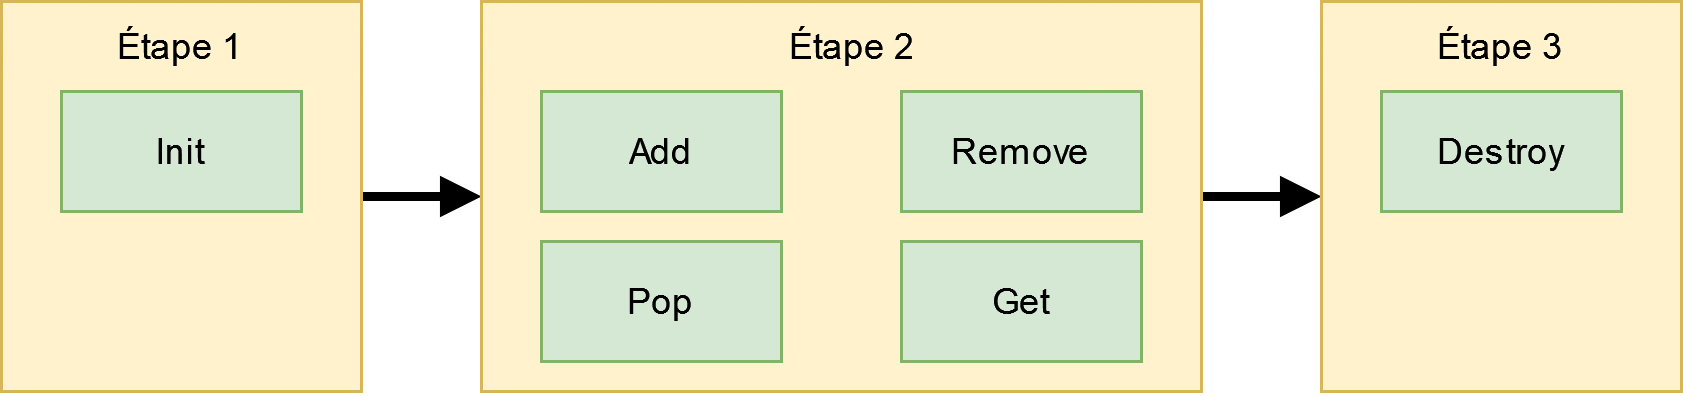
\includegraphics[width=0.9\textwidth]{img/combinator_steps_decl.png} 
	\end{center}
	\caption{Exemple de données entrée dans la partie combinaison de la librairie}
	\label{fig:combinainaison_decl_example}
\end{figure}

Les ordres d'appel de méthodes générés maintiendront toujours deux caractéristiques (comme vu sur la figure \ref{fig:combinainaison_util_example})
\begin{itemize}
\item Les actions ne seront jamais exécutées en dehors de l'étape dans laquelle elles ont été déclarée.
\item Au sein de l'étape, une action peut être utilisée un nombre arbitraire de fois, en combinaisons avec toutes les autres action déclarée au sein de cette étape.
\end{itemize}

\begin{figure}[ht]
	\begin{center}
		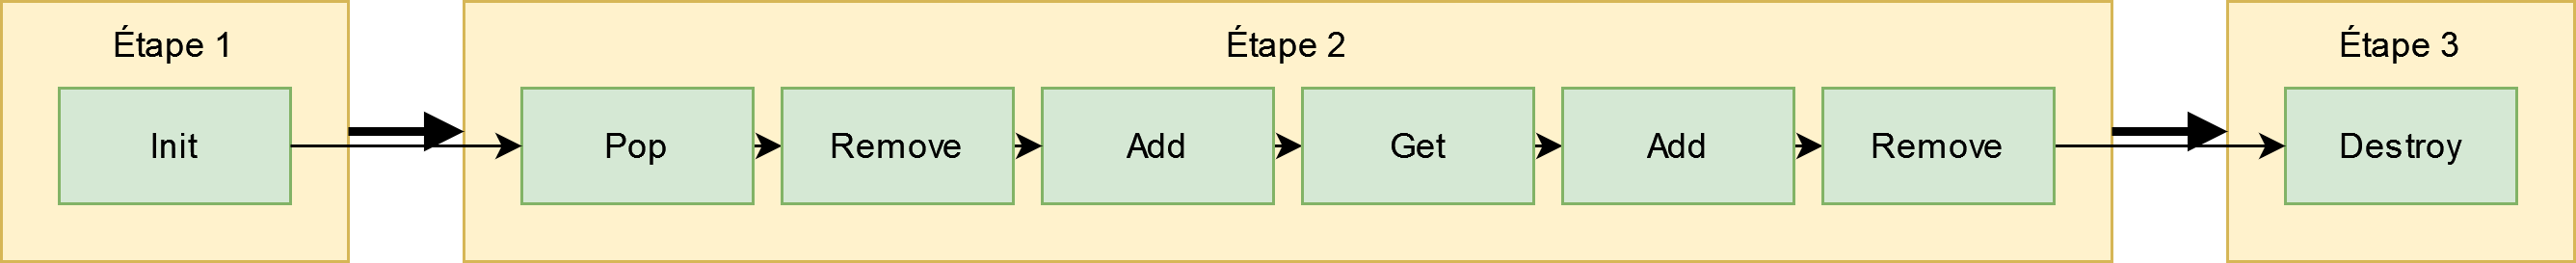
\includegraphics[width=0.9\textwidth]{img/combinator_exec.png} 
	\end{center}
	\caption{Exemple de combinaisons générée par la libraire}
	\label{fig:combinainaison_util_example}
\end{figure}

\begin{figure}[ht]
% note : step: premier tab testé, deuxième: réf
\begin{python}
from correcteur.steps.StepsRunner import StepRunner
from correcteur.steps.Step import Step

runner = StepRunner(stop_on_first_error=True)

runner.add_step(Step(
	[lambda: 0],
	[lambda: 0])
)
runner.add_step(Step(
	[lambda: 0, lambda: 1/0],
	[lambda: 0, lambda: 0])
)
runner.add_step(Step(
	[lambda: 0],
	[lambda: 0])
)

runner.compare_codes(reporter)
\end{python}
	\caption{Utilisation de la librairie en mode combinaisons}
	
	\textit{Note: pour des raisons de démonstrations une erreur a été glissée dans un des appels du code testé dans la seconde étape.}	
	
	\label{fig:combinaisons_ref}
\end{figure}


% note comparé au on error
Les erreurs peuvent être détectées par la librairie de deux façons différentes:

\paragraph{En mode comparaisons,} la librairie va tester en même temps la même combinaison d'actions sur le code de référence et le code testé.
Dans l'exemple (Fig \ref{fig:combinaisons_ref}), les appels testés sont dans le premier tableau passé aux objets "Step" et les appels de référence sont dans le deuxième tableau passé.
La librairie va  comparer les retours de fonctions ainsi que les erreurs remontées au code de référence lors des tests.
Si le retour d'un appel de référence n'est pas, exactement, le même que le retour du code testé, une erreur va être logguée.
Si l'exception levée par le code testé n'est pas la même que celle levée par le code de référence ou bien que le code testé a levé une exception et pas le code de référence une erreur va également être logguée. 


\paragraph{En mode solo,} la librairie va également exécuter uniquement le code testé, sans code de référence.
Pour utiliser cette partie de la libraire sans code de référence et se baser uniquement sur les erreurs remontées pour détecter les fautes, if faut simplement passer "\textbf{None}" ou ne rien mettre comme second argument.
Dans ce mode-ci, les erreurs seront détectées grâce aux exceptions lancées.
Chaque exception lancée sera logguée et remontée.


%stop_on_first_error
Un problème récurrent qui a été noté lors du test de cette fonctionnalité de la librairie est l'inondation d'erreurs dans le logguer lorsqu’une erreur est détectée.
Cela est dû au fait qu'une erreur peut, dans bien des cas, être déclenchée par de nombreuses combinaisons d'actions différentes.

Dans le cas de l'exemple cité plus haut, si une erreur et présente dans une des actions de la dernière étapes, toutes les combinaisons d'actions incluant cette action vont être comptées comme en échec et, à cause de cela, toutes celles-ci seront ajoutées dans le logger d'erreurs.
Cela va générer beaucoup d'erreurs remontées à l'étudiant, pour aucune valeur ajoutée.
Si d'autres erreurs sont détectées, elles ne seront probablement pas vues, car noyées dans le bruit généré par cette première erreur.

La solution qui a été adoptée a été d'ajouter au \textit{Runner} une option pour que l'évaluation cesse après une erreur détectée.

Dans le cas où plusieurs erreurs sont présentes dans le code, une seule sera remontée par exécution et l'étudiant devra les corriger au fur et la mesure de ses soumissions.
Ce compromis a été fait, car une re-soumission n'est pas très couteuse et ne pénalise pas l'étudiant.
En plus, ce retour limité à une seule erreur ne diminue que de peu la pertinence du retour donné à l'étudiant, car toutes les erreurs de son implémentation seront détectées sur les multiples soumissions de son code.
  

%nice name
Lorsque la combinaison d'actions dans les étapes détecte une erreur, celle-ci sera remontée au code parent via un logger dédié.
Celui-ci recevra, quand aucun nom n'est précisé, que le numéro de l'action qui a raté (par manque d'information disponible).
Afin de permettre un feedback plus lisible et intéressant pédagogiquement aux étudiants, un paramètre optionnel, \textbf{"nice\_names"} , a été créé.
Celui-ci est un tableau qui contiendra un nom lisible pour l’action passée à l'étape.
L'exemple de la figure \ref{fig:combinaisons_ref} peut être modifié comme démontré dans la figure \ref{fig:combinaisons_ref_name} pour inclure des noms lisibles.

\begin{figure}[ht]
% note : step: premier tab testé, deuxième: réf
\begin{python}
from correcteur.steps.StepsRunner import StepRunner
from correcteur.steps.Step import Step

runner = StepRunner(stop_on_first_error=True)

runner.add_step(Step(
	[lambda: 0],
	[lambda: 0],
	nice_names = [
		"init"
	])
)
runner.add_step(Step(
	[lambda: 0, lambda: 1/0],
	[lambda: 0, lambda: 0],
	nice_names = [
		"add",
		"remove"
	])
)
runner.add_step(Step(
	[lambda: 0],
	[lambda: 0],
	nice_names = [
		"destroy"
	])
)

runner.compare_codes(reporter)
\end{python}
	\caption{Utilisation de la librairie en mode combinaisons avec des noms lisibles}
	
	\textit{Note: pour des raisons de démonstrations une erreur a été glissée dans un des appels du code testé dans la seconde étape.}
	
	\label{fig:combinaisons_ref_name}
\end{figure}

L'ajout de ces noms va modifier le retour fait aux étudiant de, par exemple:
\begin{center}
Une erreur a été trouvée après avoir exécuté les étapes suivantes: 1 -> 1 -> 2
\end{center}
à
\begin{center}
Une erreur a été trouvée après avoir exécuté les étapes suivantes: init -> delete -> add
\end{center}

Ces noms donnés aux fonction sont liés, un à un, entre les tableaux d'actions et le tableau de noms.
Le premier nom correspondra à la première action, le deuxième au deuxième et ainsi de suite.


\newgeometry{a4paper,left=1in,right=1in,top=1in,bottom=1in,nohead}
\begin{landscape}
	\section{Récapitulatif des méthodes de tests}
	%tableau récapipitlatif de tte les techniques, de leurs avantages et inconvé&nient et si elles ont été sélectionnées :D 
	\begin{tabularx}{1\linewidth}{>{\centering}p{0.2\textwidth}||p{0.55\textwidth}|p{0.55\textwidth}|p{0.2\textwidth}}
	Technique & Avantage(s) & Défaut(s) & 
	Utilisée  \\
	\hline 
	\hline   
	Tests par propriétés & 
	\begin{itemize}
	\item Couverture des entrée très complète
	\item Cas problématique minimisé par l'oracle
	\end{itemize}
	 &
	\begin{itemize}
	\item Propriété longue à écrire pour être utiles
	\item Non générifiable
	\end{itemize}
	 & Non \\ 
	\hline   
	Injection de fautes &
	\begin{itemize}
	\item Test quasi complet du code de récupération
	\item Branches complexes à atteindre atteintes
	\end{itemize}
	 &
	\begin{itemize}
	\item Uniquement utile en environnent réel
	\item Peu efficace en environnement simulé, avoir des interfaces modifiées vers l'extérieur est plus simple
	\end{itemize}
	 & Non \\ 
	\hline   
	Fuzzing en boite noire &
	\begin{itemize}
	\item Utile pour explorer  automatiquement
	\item Très peu de temps de préparation des tests
	\end{itemize}
	 & 
	\begin{itemize}
	\item Fortement dépendant des entrées initiales
	\item Peu efficace
	\end{itemize}
	 & Non \\ 
	\hline   
	Fuzzing en boite blanche & 
	\begin{itemize}
	\item Couvertures très complètes des branches
	\end{itemize}
	 & 
	\begin{itemize}
	\item Instrumentation complète de l'interpréteur obligatoire
	\item Ré-adaptation nécessaire pour chaque version mineure du language si ne travaille au niveau de l'exécution du processus dans le kernel du système
	\item Très grand et complexe à mettre en place 
	\end{itemize}
	 & Non \\ 
	\hline   
	Fuzzing en boite grise & 
	\begin{itemize}
	\item Auto-génération des entrées initiales possibles
	\item Couvertures des branches correcte
	\item Couverture basique des branches rapidement obtenues
	\end{itemize}
	 & 
	\begin{itemize}
	\item Couvertures des branches parfois moins complète
	\end{itemize}
	 & Oui \\ 
	\hline   
	Combinaison d'appels & 
	\begin{itemize}
	\item Cherche des états internes mauvais
	\item  Interprétation des résultats aisée
	\end{itemize}
	 & 
	\begin{itemize}
	\item Complexité à contrôler
	\item Arguments d'entrée des appels fixés
	\end{itemize}
	 & Oui \\ 
	\hline 
	\end{tabularx}
\end{landscape}
\restoregeometry 
% =====================================================================



\chapter{Contributions}
% mémoire de RECHECHE pas d'application
%description globale combi + fuzzer => lib + docker
La majeure partie de la réalisation du mémoire a été consacrée à la création et à l'intégration d'une librairie de test automatique suite aux recherches faites sur ceux-ci.
La librairie crée est découpée en plusieurs éléments.

Le premier est composé des implémentations des techniques de correction que sont le fuzzing et la combinaison d'exécutions.
La seconde est l'intégration de ceux-ci dans un environnent Inginious prêt à être utilisée.

Cette partie du document est dédiée à l'analyse de détails d'intégration notable ou intéressants, à l'examen de l'efficacité de a solution et a une critique de ce qui a été développé en regardant de plus près ses limitations.



\section{Intégration}
% pret a être facilement utilisé dans inginious 
% peu de code nécéssaire
% template
%flexibilité
Au fil de ce mémoire, l'objectif principal qui a été poursuivi a été d'arriver à une intégration fonctionnelle et robuste dans Inginious dont l'utilisation est simple et claire.
La petite quantité de code nécessaire à créer  de nouveaux tests a également été un facteur poursuivi afin de permettre un déploiement rapide pour, par exemple, la création de nouveau cours dans la plateforme Inginious.
certains points de l'implémentation et l'intégration ont reçu une attention particulière ou ont nécessité des décisions spécifiques.
Cette section est dédiée à ceux-ci, aux conséquences qu'ils ont eu ainsi qu'aux modifications de design que certaines des contraintes découvertes ont impliqué.

\subsection{Gestion des erreurs}
Une grande attention a été portée sur la gestion des erreurs remontées à l'étudiant.
En effet, celle-ci sont capitales pour que l'étudiant soie en mesure de comprendre ce qui n'a pas fonctionné ou ce qui est problématique et puisse y remédier.

Il est également nécessaire d'avoir une structure mise en place assez flexible pour permettre de l'étendre avec n'importe quel type d'erreur ou de besoin futur.

La structure qui a été adoptée a été une structure de logger d'erreur générique à buffer interne.
L'objet Python de base, tel que décrit dans le code suivant, est conçu pour être étendu.


\begin{python}
from correcteur.feedback.ErrorLog import ErrorLog

class ErrorReporter:
    def __init__(self):
        self.errors = []

    def add_error(self, error: ErrorLog):
        self.errors.append(error)

    def get_output(self) -> [str]:
        raise NotImplementedError

    def get_text_output(self) -> str:
        res = ""

        if len(self.get_output()) != 0:
            for line in self.get_output():
                res += line
                res += "\n"
        return res
\end{python}



Il a été considéré comme plus intéressant d'avoir une structure générique améliorable facilement en divers loggers spécialisés plutôt qu'un seul logger qui serait difficile à maintenir, à étendre, à intégrer et à débugger.


Pour des facilités d'utilisation de la librairie, un logger textuel simple, étendant l'objet "ErrorReporter" de base est fourni.
Celui-ci est visible dans le code suivant.


\begin{python}
from correcteur.feedback.errorRepporter import ErrorReporter


class TestRepporter(ErrorReporter):

    def get_output(self) -> [str]:
        res = []
        for error in self.errors:
            res.append(
                "[{method}] {msg} (Error: \"{error}\")".format(
                    error=error.error,
                    method=error.methode,
                    msg=error.message))
        return res
\end{python}

Ce rapporteur, très simple, se content de mettre l'erreur levée dans une string formatée de façon intelligible pour l'étudiant.
Son gros défaut est qu'il compte sur le fait que les erreurs qui lui sont reportée sont déjà complètement utilisables comme feedback et ne fait aucun traitement supplémentaire des inputs qui lui sont données afin de les améliorer ou de les rendre plus compréhensibles.


Un exemple type de ce logger dans un des algorithmes de détection de faute peut être observé dans le code suivant.

\begin{python}
from correcteur.feedback.ErrorLog import ErrorLog
from correcteur.feedback.errorRepporter import ErrorReporter

# testing fait et les erreurs detectee sont
# collectees dans le tableau "fail"

for i in fail:
	reporter.add_error(ErrorLog("fuzzer", i[1],
		"the fuzzer broke the" \
		" code  (inputs: {})".format(i[0])))
\end{python}



Comme vu dans la figure précédemment mentionnée, le logger est passé comme argument à chaque exécuteur.
Cela permet, si nécessaire, de passer un logger personnalisé / spécialisé / adapté différent à chaque structure afin de personnaliser un maximum la remontée d'erreur et donner un retour le plus pertinent possible à l'étudiant.

\subsection{Ajout d'un type de donnée}

%yeay ez pz
Comme pour la gestion des erreurs, l'ajout d'un nouveau type de donnée dans le fuzzer a été conçu pour être très simple à faire.
Un type de donnée est représenté par un objet qui a plusieurs rôles quant à la gestion de la vie de ce type dans le fuzzer.
C'est celui-ci qui va s'occuper de:
\begin{itemize}
\item les créer de façon aléatoire
\item les muter
\item sélectionner les cas spéciaux à partir des tokens statiques trouvés dans le code source
\item les créer à partir des cas spéciaux
\end{itemize}

Pour en créer un nouveau, il va simplement être nécessaire d'étendre la classe input (\textit{correcteur/fuzzing/input/input.py}) au sein du même module.
Comme mentionné précédemment, la classe input contient tout ce qui est nécessaire pour permettre au fuzzer de travailler avec le type de donnée représenté par ses classes enfants.
\begin{python}
class Input:
    def __init__(self):
        pass

    def integrate_by_type(self, candidates):
        """
        Will take a list of candidates as an input
        and integrate the compatibles one as internal
        base seeds
        :param candidates: the set of potential candidates
        """
        raise NotImplementedError

    def get_special_cases(self):
        """
        :return: an array of seed for this type of
        	runner that represent base special cases
        """
        return []

    def get_random(self):
        """
        :return: a new, completely random seed for
        	this input
        """
        raise NotImplementedError

    def can_mutate(self):
        """
        Will return if the type is able to be mutated
        """
        return True

    def mutate(self, value):
        """
        :param value: the base input
        :return: a new , mutated by a bit, value
        """
        raise NotImplementedError

    def is_valid_type(self, candidate):
        """
        :param candidate: the python object that is
        	going to be analysed
        :return: True if the given object match the
        	type of this one
        """
        raise NotImplementedError
\end{python}

Une fois le nouveau type créé, il ne reste plus qu'à l'ajouter à la fonction qui fait la comparaison entre les annotations présentes sur la fonction testée et les types tels qu'implémentés ici.
Faire ce rajout est trivial car, comme montré dans le code suivant, la fonction est très simple dans sa conception.

\begin{python}
def get_type_from_str(name):
    if name == "int":
        return Int()
    if name == "float":
        return Float()
    if name == "bool":
        return Bool()
    if name == "str":
        return Str()

    if name == "List[int]":
        return List(internal_type=Int())
    if name == "List[float]":
        return List(internal_type=Float())
    if name == "List[bool]":
        return List(internal_type=Bool())
    if name == "List[str]":
        return List(internal_type=Str())

    raise NotImplementedError()
\end{python}

\textit{Note importante à propos de cette fonction: le type "List" vu dans celle-ci n'est \textbf{pas} le type list primitif de Python mais bien un type de donnée implémenté comme les autres.}

%types composites
Les types composites (composé de plusieurs sous-types) sont supporté, comme, par exemple, l'implémentation du type "List" le démontre.
Ceux-ci marchent de la même façon que leurs homologues simples, à la différence près qu'ils vont déléguer certaines taches et informations aux types qu'ils contiennent.
Pour qu'un type composé soit pris en compte, il est nécessaire d'ajouter toutes ses formes dans la fonction décrite plus haut pour qu'il soit possible de l'utiliser automatiquement au bon endroit lorsque l'utilisation d'annotation de types est utilisée.


%\subsection{Interface unifiée}

%TODO expliquer l'interface unifiée vite fait

\subsection{Intégration dans Inginious}

%décrire l'intégration globale, ce qui a été fait
Pour faciliter une intégration rapide et sans problèmes dans la plateforme Inginious, un fichier Docker pour créer un conteneur de vérification Inginious a été créé.
Une fois ce conteneur créé sur la machine hébergeant Inginious, il suffit de relancer Inginious puis d'aller sélectionner l'environnement "python3-correcteur" dans la tâche.

Ce fichier de construction docker se base sur l'environnent Python 3 de base et ajoute la librairie développée dans le cadre de ce projet sur le path Python afin de permettre une importation aussi simple.
Par exemple, que ceci:

\begin{python}
from correcteur.fuzzing.fuzz import fuzz
\end{python}

Le dockerfile est composé comme suit:
\begin{python}
FROM ingi/inginious-c-python3
LABEL org.inginious.grading.name="python3-correcteur"


RUN pip3 install astunparse
RUN mkdir -p /python
COPY correcteur /python/correcteur
ENV PYTHONPATH="/python:\${PYTHONPATH}"
\end{python}


Pour aider à l'intégration du projet dans Inginious, un cours d'exemple a été créé et contient un exemple des quatre modes possibles:
\begin{itemize}
\item fuzzer avec fonction de validation
\item fuzzer sans fonction de validation
\item combinateur avec code de référence
\item combinateur sans code de référence
\end{itemize}
Ces quatre modes donnent leur feedback de la même façon: écrire le feedback sur la sortie standard et se servir de cet output comme message de retour.
Ce comportement est, bien sur, hautement personnalisable et est adaptable facilement aux modèles personnalisés de feedback Inginious.

\section{Efficacité}

Ce projet a été réglé pour être réalistement utilisable dans le contexte de l'enseignement.
Pour ce faire, certaines concessions  ont été faites et certaines décisions arbitraires ont été prises.
Celles ci-sont l'objet de cette section.

\subsection{Type d'erreurs détectées}

%combinator => bad internal state
%fuzzer => bad input handling (mostly) and shitty bugs
% qu'est ce qui est pas trouvable

Les deux approches utilisées sont particulièrement adaptées pour trouver certains types de problèmes.
Ceux-ci couvrent une certaines parties des erreurs possibles mais pas toutes.

\paragraph{Le fuzzer} sera particulièrement bon pour trouver des cas particuliers non supporté sur les entrées.
De par sa nature et le fait qu'il est, dans ce cas-ci, fait pour prendre comme entrées de base les nombres hard-codés du programme ainsi que les cas particuliers de chaque type, il va être très efficace pour réussir à déceler les bugs d'entrées non saines.
L'utilisation principale faite de celui-ci pour trouver les problèmes avec les parties de programme en contact avec les entrées utilisateurs abonde dans ce sens (comme, par exemple le "Security Development lifecycle" créé par Microsoft \cite{howard2006security}).

\paragraph{L'algorithme de combinaison d'appels} va être particulièrement utile pour trouver des combinaisons d'action qui vont créer un état interne du programme indésirable.
Tous les états problématiques ne seront pas trouvés, seuls ceux qui résultent en une erreur détectable par le programme de test.
Celui-ci reste limité par son ignorance des paramètres et sa concentration sur les appels (les paramètres sont fixés pour tous les appels).

\paragraph{Les problèmes non trouvés} peuvent être multiples.

Les bugs qui ont besoin, pour être déclenchés de combinaisons d'appels et de paramètres spécifiques vont être très difficiles à déceler.
Globalement, plus un problème présent dans un programme a besoin d'une grande combinaison d'appels ou d'un nombre élevé de paramètre pour arriver, plus difficilement il sera décelé par les approches de test automatique décrites dans ce document.
Une façon de palier, en partie, à ce problème de rajouter certaines analyses statiques et des conventions fortes pour éviter que ces situations problématiques complexes puissent apparaître.

Les problèmes qui, pour être détectés ou apparaitre dépendent d'évènement externe non anticipé sont également plus difficiles à déceler avec les approches prises ici.
L'environnent étant fort contrôlé, ajouter des tests par l'injection de fautes ne serait pas fort intéressant.
Il est, en effet, possible dans ce cas-ci, d'empoisonner les interfaces avec ces évènements extérieurs pour simuler le problème (en pratique, cela peut être fait avec le combinateur).
Une autre approche possible est d'utiliser de l'injection de fautes.

\subsection{Valeurs par défaut}
% valeurs raisonable par défaut sinon c'est la meeeeeeeeeeeeeerde
Un des choix arbitraire qu'il a fallu faire sont toutes les valeurs par défaut utilisées.
Celles ci sont très importantes car, si bien réglées, permettent d'utiliser plus facilement le projet en devant développer moins, ce qui est un des objectifs de ce mémoire.

Ces valeurs par défauts ont été trouvées empiriquement en utilisant un un exemple représentatif souvent utilisé dans les cours d'algorithmique (une implémentation partiellement fausse de Dijkstra a été utilisé).
La machine sur laquelle ces tests ont été faits est relativement puissante (cpu: AMD ryzen 7 5800x).
Cet effet a été pris en compte en divisant le résultat obtenu par la fréquence de la machine hôte et multipliant le chiffre obtenu par 2.5Ghz (un cpu de serveur moyen de gamme actuel, par exemple le AMD EPYC 7502, atteint ces performances).
Ce nombre a finalement été arrondi vers le bas pour rajouter un peu de marge.

\section{Distribution}
% 1/2 page lien vers repo et quelques info sur le proto
Le code développé est mis à disposition via deux git publiques:
\begin{itemize}
\item \url{https://git.ortegat.com/pierre/Memoire_unamur}
\item \url{https://github.com/reirep/unamur-tests-python-auto}
\end{itemize}

Celui sur "ortegat.com" est celui qui a été principalement utilisé et le clone fait de celui-ci sur Github est là pour la pérennité du code.

Sur ce repo git, une branche "\textit{ecrit}" contient ce document.

Quatre éléments sont intéressants à connaître pour aborder ce repo.

Tout la librairie est contenue dans le dossier "\textit{correcteur}" et celui-ci est découpé en composants haut niveau.
Il est composé:
\begin{itemize}
\item du dossier feedback qui contient tout le code nécessaire au logging et remontage des erreurs et messages vers les étudiants.
\item du dossier fuzzing qui contient le fuzzer en greybox
\item du dossier steps qui contient l'algorithme de combinatoire
\end{itemize}

Le cours d'exemple qui a été produit pour aider à l'utilisation de la libraire se trouve dans "\textit{ressources/www/inginious/tasks/autocorrect}".
Celui-ci est conçu pour être simple à suivre et comprendre.

Le \textit{Dockerfile} qui permet de construire un environnent Inginious prêt à être utilisé.

le fichier \textit{main.py} qui contient quelques exemples d'utilisation simple de la libraire.

\subsubsection{Démarrage rapide}

Pour mettre en place rapidement ce projet dans un Inginious déjà existant, il est simplement nécessaire de faire un "\textit{make docker}" à la racine du projet.
Un docker (et environnent de test Inginious) du nom de "python3-correcteur" va être créé et, après un redémarrage d'Inginious, pourra être utilisé directement dans les cours.
Pour voir des exemple d'intégrations, regarder le cours de test présent dans le dossier "\textit{ressources/www/inginious/tasks/autocorrect}".

\chapter{Discussions}

Les techniques sélectionnées au fil de ce mémoire ont été implémentées mais n'ont pas été testées sur le terrain au delà du projet d'exemple.
Cette section va se concentrer sur plusieurs approches possibles pour tester ce qui a été produit ainsi que l'identification des limitations possibles.

Pour commencer, les bénéfices apportés par un telle approche seront explorées.
Ensuite, certaines expériences ont été imaginées pour tester quelles seraient l'approche idéale avec les outils disponibles et si la librairie produite fait partie de ces outils.
Dans la foulée, une attention toute particulière sera apporté à la constitution des groupes d'étude, certains détails rendant celle-ci intéressante.
Enfin, les limitations actuellement connues / identifiés de ce qui a été produit seront explorées.

\section{Amélioration de l'apprentissage}
% lol, ca va aider à faire plus d tests auto, donc on va attraper des "avantages" 

% potentiel d'améilloration de l'apprentissage derval2015automatic
L'optique de recherche de ce mémoire est directement lié à la quantité d'exercice disponible à un étudiant pour un cours donné et à la qualité de la correction qui lui est disponible.
Les avantages d'avoir un cours bien réalisé sur une plateforme d'apprentissage en ligne avec correction automatique s'appliquent également ici.
%Les remarques faites ici sont applicables également aux cours construits dans le cadre d'un MOOC.

% apprentissage à la demande
L'apprentissage, l'application de la matière et l'entrainement à la demande permettent aux étudiants de pouvoir réaliser et étudier le cours quand ils le désirent.
Il n'est plus nécessaire de jongler avec une armée d'assistants et de travaux pratiques, tout en gardant une qualité d'apprentissage très proche de l'ancien système de travaux pratique en petits groupes en classe \cite{derval2015automatic}.

% autant d'essais que nécéssaires
Les étudiants arrêtent d'êtres limités dans le temps mais également en nombre d'essais.
Si un profil particulier à besoin de 200 essais pour comprendre la façon dont une partie de la matière fonctionne, cela devient possible, il n'est plus limité par les ressources humaines limitées de son lieu d'enseignement.
Les profils pour lesquels les travaux pratiques en journée ne conviennent pas pourront en toute liberté les faire quand ils le désirent, à toute heure du jour et de la nuit.

% feedback personalisé (feedback enrichis  Derval2022 )
L'utilisation de plateforme de correction en ligne permet de rajouter un élément personnalisé à la correction et un retour enrichi qui permettra à l'étudiant de progresser plus efficacement dans son appropriation du cours \cite{Derval2022}.

% retour pour le prof sur les perfs élèves Hormaux 
Un autre aspect de ce genre d'approche est que cela donne une idée précise du niveau du groupe et cela permet au titulaire d'avoir un retour très précis sur l'état de la classe.
% plus facile d'identifier les problèmes d'apprentissage du groupe Martin
Ce genre d'approche permet au prof de donner son cours de façon plus dynamique en fonction de ce que la plateforme de correction lui rapporte \cite{Martin}.
En cas de lacune particulière remarquée, il devient possible d'adapter ou de repasser sur un point de matière en particulier.


\section{Contribution de la librairie à la réussite}
Cette section se concentre sur plusieurs expériences et approches qui pourraient être mises en place afin de tester précisément l'impact de ce qui a été produit dans la cadre ce mémoire sur l'expérience et l'apprentissage étudiant.
Comme c'est une approche théorique et qu'il est nécessaire de pourvoir d'adapter à la réalité du terrain, plusieurs solutions ont, à chaque fois, été proposées.


\subsection{Protocoles de test}

% double aveugle
%% éviter d'influencer
Un des éléments les plus importants pour la réalisation de cette expérience est que, peu importe le support, elle soit réalisée en double aveugle.
Comme ce qui est testé ici est uniquement la partie cachée de la plateforme de correction, il est tout à fait possible de mettre en place une expérience complètement opaque aux participants (par participants, il est entendu les étudiants \textit{ainsi} que le corps enseignant).

Éviter des phénomènes qui pourraient se produire, tels qu'un étudiant qui voit sa motivation modifiée, car il est sur une plateforme différente de ses congénères ou, car il a eu un accès spécial qui lui a été donné par un assistant (qui pourrait simplement être une autre version du test), est capital car ceux-ci ne sont pas des phénomènes désirables pour  la pertinence des résultats.

Au même titre, il est important que le personnel enseignant, et plus particulièrement celui qui va se charger de la correction de l'examen final, ne sache pas quel participant fait partie de quel groupe.
de nouveau, pour éviter qu'un biais quelconque n'apparaisse.
Ne pas connaitre les noms des étudiants lors de la correction finale n'est pas suffisant car chaque étudiant ayant un style propre.
Le personnel enseignant pourrait, même inconsciemment, associer le style personnel de l'étudiant à celui-ci et donc à voir un biais de correction.

Avec la plateforme Inginious il est possible que cette décision soit gérée par la plateforme en elle même et que les résultats de l'expérience ne soient divulgués qu'une fois le cours clôturé.
Dans ce cas ci, cette approche est beaucoup plus pertinente.

\paragraph{Deux façons de tester} ont été envisagée et l'application de l'une ou l'autre dépend du type d'exercice qui est testé.
Chacune des façons utilise une des parties de la librairie et, idéalement, les deux seraient testés en même temps sur deux exercices différents avec les groupes mixés d'un test à l'autre.
Celles-ci vont être passées en revue afin de permettre une application optimale des deux combinaisons de tests décrites ci-après.

% unit vs fuzzig vs pas d'accès
La première est concentrée sur la partie fuzzer et s'adresse plutôt à un exercice dont les tests se concentrent sur une seule interface.
En effet, les limitations du fuzzer étant ce qu'elles sont, le fuzzer ne sait pas tester de combinaisons d'appels différents; uniquement des combinaisons du même appel avec des entrées différentes.
Le test serait divisé en quatre groupes.
\begin{enumerate}
\item le premier serait corrigé exclusivement par le fuzzer.
\item le second serait corrigé exclusivement par des tests unitaires écrits à la main adaptée spécialement pour l'exercice.
\item le troisième serait une combinaison des deux. Les tests unitaires seraient d'abord exécutés puis, si ceux-ci n'ont rien trouvé, le reste du temps d'exécution disponible dans le runner Inginious serait utilisé pour le fuzzer (qui, bien sur, serait paramétré pour prendre moins de temps et faire moins de tests pour accommoder le temps réduit. Utiliser les valeurs par défaut dans ce cas-ci n'est pas adapté).
\item le quatrième  devrait se débrouiller sans la plateforme de correction automatique, comme groupe de contrôle.
\end{enumerate}
Note qu'il peut être difficile de faire un test en double aveugle dans lequel un groupe n'aurait pas accès du tout à la plateforme de correction mais certaines circonstances le permettraient, par exemple, dans le cas de cours donné à distance ou de petits groupes qui n'ont pas de contacts entre eux.
Si cela n'est pas possible, le quatrième groupe peut être supprimé et le second groupe, celui qui utilise exclusivement les tests unitaires et rien de la librairie, peut être considéré comme le témoin.

% unit vs combi vs pas d'accès
La seconde possibilité découpe des participants en quatre groupes aussi, mais au lieu d'avoir un groupe qui va être corrigé par le fuzzer et un groupe qui va être corrigé par les tests unitaires et le fuzzer,  il y aura un groupe qui va être corrigé par les tests combineurs et un groupe  qui va etre corrigé par les tests unitaires et les tests combineur.
Cet arrangement-ci est plus adapté l'exercice testé est quelque chose sur lequel on teste des combinaisons d'appel (comme mentionnée précédemment, par exemple, une liste liée)

\subsection{Constitution des groupes d'étude}
%% attention le groupe doit etre assez grand (idéalement, la taille théorique de chaque groupe > 30 pour etre stat significant
Pour les partitions en groupe proposé juste avant, il est nécessaire que plusieurs éléments soient présents afin d'être sûr que les résultats obtenus soient exploitables.

L'attribution des participants dans les groupes se doit d'être particulièrement surveillé afin de guarantir des groupes cohérents.
La répartition est envisageable de trois façons différentes qui vont être détaillées dans les paragraphes suivants.

\paragraph{Une répartition aléatoire} a quelques avantages non négligeables \textit{si} le groupe de participants à découper en groupe est assez grand.
En effet, ce mode de répartition permet de garantir qu'un groupe ne possédera pas de caractéristiques particulières distincte des autres.
%Cela est d'application uniquement si le groupe est assez grand.
Dans le cas où le groupe n'est pas assez grand (cette limite dépendant du nombre de facteurs à contrôler: plus il y en a plus il faut un grand groupe pour que la répartition au hasard marche) il y a un risque qu'un groupe aie une caractéristique distinctive ce qui rendrait les résultats inutilisables, car cette caractéristique pourrait être la justification de la moindre observation faite.

% attribution hashée
%% pas de biais dans l'attribution des groupes
\paragraph{Une répartition hashée} a les mêmes avantages et défauts que la répartition aléatoire, à un détail près.
Assigner les participants sur base d'un hash qui leur est lié permet que le système les répartisse les participant de façon pseudo aléatoire crédible tout en améliorant le double aveugle.
Les contrôleurs / le personnel enseignant n'ayant pas le hash, l'opacité de l'expérience n'en est qu'argumentée.
Utiliser un hash plutôt qu'une assignation aléatoire permet de réellement découpler les résultats du profil initial sans pour autant perdre le lien.


% ou bien atriution en répartition en groupes équitable d'après les groupes spotté par un classificateur ml \cite{Hormaux}
\paragraph{Une répartition sur base des résultats précédents ou d'un test de positionnement} peut être utilisée afin de garantir une répartition en groupe plus uniforme.
Dans un premier temps, un élément classificateur (résultats précédents, test de placement, ...) classerait les étudiants par profil de performances \cite{Hormaux} et dans un second temps, l'expérience commencerait avec des groupes composés de tous les types de profils, répartit de façon homogène.
L'avantage de cette approche est qu'elle marche aussi avec de plus petits groupes et ne laisse pas la chance d'une répartition uniforme au hasard.


\section{Limitations}

% certains détail d'impl qui sont utiles à savoir

\begin{center}
Cette librairie n'est pas parfaite.
\end{center}

% best effort
% blind spot
% limité par le temps d'execution
Elle a été conçue de façon à optimiser plusieurs choses.

Le temps de correction doit être assez court pour qu’au moment de son retour, la réponse soit encore pertinente.
Les tests automatiques ne sont pas omniscients et peuvent avoir des zones aveugles en fonction de la situation.
Son développement a été étalé sur une période limitée et les approchées sélectionnées ont tenu compte de ce facteur.


Tous ces éléments combinés ont pour conséquence que cette librairie, bien que conçue pour tirer le meilleur de certaines tactiques de détection de problèmes, n'est pas la solution parfaite mais une approximation qui se veut le plus proche de celle-ci.

Certaines des limitations sont traitées plus en profondeur au fil de la section suivante.


\subsection{Tests d'objets génériques}
% créer à la volée des objets génériques n'a pas d'intéret: cela conformerait au code et non a la spec du code : aka ca prendrait les erreurs dans l'objet et les valideraient
Une proposition qui  a été écartée qui aurait pu, dans d'autres circonstances que celle ce projet être utile, est la création à la volée d'objets correspondant à ce qui est  attendu par le code testé en se basant sur les erreurs retournées par celui-ci.
Le "duck typing" de Python permet de faire cela sans trop de difficulté (Deux objets différents en Python ayant les mêmes signatures de méthodes et  les mêmes noms de variables sont considérés comme étant de même type. Pour être plus précis, les deux types sont considérés comme identiques.).

Le problème est que, au lieu de créer à la volée l'objet qui est \textit{censé} être passé au programme, il sera construit systématiquement l'objet qui correspond parfaitement à ce que le programme accepte, que ça soit juste ou non.
Ces objets créés ne correspondront pas à ce qui va, lors de l'utilisation du programme, être réellement passé à celui-ci.
Cette technique valide uniquement que le programme accepte des objets qui sont parfaits pour ce qu'il est non ce qu'il \textit{devrait être}.



\subsection{Résolution des branches}

% limitations dues à l'arret du programme pour une résolution statique
% => extension problème d'arret
Résoudre statiquement toutes les expressions présente dans le programme testé permet au fuzzer de partir sur une base d'entrées saines et pertinentes.

Les plus faciles à détecter sont les nombres magiques présents dans le programme (un nombre magique est, dans le contexte d'un programme, une constante basée sur rien / peu de choses que le développeur a utilisé).
Les expressions simples suivent rapidement derrière car un algorithme de parcours et une implémentation de calculatrice saura les résoudre.

Un des problèmes qui va très vite être rencontré lorsque de plus grandes expressions vont être considérées, est qu'il est impossible de statiquement affirmer si une boucle quelconque dans un programme va se finir et si oui, si c'est dans un temps raisonnable.
Ce problème peut être vu comme une application du problème d'arrêt \cite{burkholder1987halting} dans lequel la boucle est un programme inclus dans un programme plus grand.
Cette idée qu'une boucle peut être une application du problème d'arrêt peut être étendue à n'importe quel groupe d'instruction, ce qui rend l'exécution d'un analyseur statique impossible pour les expressions plus complexes comprenant des structures de contrôle et non uniquement des mathématiques simples.

\paragraph{Un parseur de code générique} a été développé pour permettre de résoudre ces instructions facilement.
Afin de rester compatible avec un maximum de versions de Python, il n'assume que très peu de choses à propos de l'environment Python dans lequel il est exécuté.
Ceci est accompli avec une récursivité générique basée sur le parseur Python.

Celui-ci peut être trouvé dans le projet dans le dossier "correcteur/fuzzing/token", nommé "\textit{universal\_magic\_token\_finder.py}".   


\subsection{Détection automatiques du type d'arguments}
Une détection automatique, sans les annotations, du type d'argument qu'une fonction doit recevoir a été envisagé mais a été mis de côté à cause du peu d'avantage que cette technique apportera pour sa complexité et sa non-fiabilité.

Plusieurs problèmes, certains liés à la façon dont Python est conçu vont empêcher cette idée de fonctionner proprement.

Le fait qu'une variable en Python puisse être de n'importe quel type et changer plusieurs fois de type au cours de sa vie va complexifier énormément la détection du type de l'argument.

Les fonctions en Python n'ayant pas le type de retour inclus obligatoirement dans la signature de la fonction, il est impossible de déduire automatiquement le type de retour de la fonction sans devoir remonte  à travers le code de cette fonction récursivement.
Pour palier cela, il sera nécessaire de contraindre logiquement résolution du type d'argument, ce qui impliquerait de prédire certaines informations sur la fonction.
Une des conséquences du typing dynamique de Python est qu'une des choses qui devrait être déduite serait de savoir si une branche serait explorée ou non.
Par exemple, si le résultat d'une condition complexe est passée à la fonction de la figure \ref{fig:condition_complexe_résolution}, déterminer statiquement le type de la sortie devient impossible sans avoir résolu la valeur du bool d'entrée, sachant que celui peut rester indéfini tant que le programme n'est pas exécuté et peut varier d'une exécution à l'autre.
Déterminer si une branche va être atteinte ou pas est une extension du problème d'arrêt \cite{burkholder1987halting}: au lieu de chercher si on va atteindre une branche particulière (celle qui mène à l'arrêt du programme), on va cherche à atteindre n'importe quelle autre branche en particulier.

\begin{figure}[ht]
% note : step: premier tab testé, deuxième: réf
\begin{python}

def problematique(a: bool):
	if a:
		return 1.0
	return "deux"
\end{python}
	\caption{Programme qui poserait un problème à la détection automatique d'argument}
	
	\label{fig:condition_complexe_résolution}
\end{figure}

Certaines fonctions étant génériques et adaptées à plusieurs types, cela rend, en plus des autres problèmes cités, la détection du type des arguments d'une fonction inutile, car il n'est pas passible de déterminer automatiquement si c'est voulu et donc si le problème trouvé avec un type particulier est pertinent et bon à signaler.



\subsection{Profondeur limitée}
% fixed / limited params combiner
La partie de la librairie dédiée au combinateur est fortement limitée par le nombre d'entrées qui lui sont fournies ainsi que la profondeur maximale l'algorithme va explorer.
Le terme profondeur est utilisé ici, car on peut visualiser les différentes combinaisons comme un arbre de possibilités.
Plus le nombre de combinaison maximum d'actions par étape est grand plus la profondeur de l'arbre de possibilités généré va être élevé).
Comme montré sur la figure \ref{fig:combinaisons_tree}, la croissance de cet arbre étant exponentielle, la taille en devient vite problématique et incalculable.

\begin{figure}[ht]
% note : step: premier tab testé, deuxième: réf
	% size tree combinaison
	\textit{$ \theta $ est le nombre d'étapes}
	
	\textit{$\phi$ est le nombre d'actions disponibles par étape}
	
	\textit{$\alpha$ est le nombre maximum d'actions exécutables par étape}
	
	$$ \text{Taille de l'arbre} = f(\theta, \phi, \alpha ) = \theta*\phi^{\alpha} $$
	
	\begin{center}
	\begin{tabular}{c||c|c|c|c|c}
	\hbox{\diagbox{$ \theta $}{$\alpha$}}
	 & 1 & 3 & 5 & 11 & 17\\ 
	\hline 
	\hline 
	1 & 5 & 125 & 3125 & 48828125 & 762939453125 \\
	\hline 
	3 & 15 & 375 & 9375 & 146484375 & 2288818359375 \\
	\hline 
	5 & 25 & 625 & 15625 & 244140625 & 3814697265625 \\
	\hline 
	11 & 55 & 1375 & 34375 & 537109375 & 8392333984375 \\
	\hline 
	17 & 85 & 2125 & 53125 & 830078125 & 12969970703125
	\end{tabular}
	\end{center}
	
	\textit{Dans le tableau, la supposition est faite que $ \phi $ vaut 5.
	Un $ \phi $ de 5 a été sélectionné car c'est raisonnablement atteignable dans une utilisation normale du projet.}
	
	\textit{Dans la formule et le tableau la limite maximale du nombre d'étapes n'est pas considérée.}
	\caption{Taille de l'arbre de combinaisons d'actions}
	
	\label{fig:combinaisons_tree}
\end{figure}

Une solution a été apportée à ce problème sous la forme d'une limite globale de longueur de combinaison générée.
Toutes les combinaisons plus longues ce quelle ci ne seront pas générées.

Dans l'implémentation actuelle elles ne seront pas juste écartées, elles ne sont pas du tout générées pour gagner en rapidité et éviter de perdre du temps à créer des entrées inutiles.



\subsection{Combinaisons de techniques}
% fuzzing into combiner => inputs limités
Une limitation connue de la partie combinatoire du projet est le manque de paramétrages des actions.
Chaque action ne peut, en effet, pas avoir de paramètre ou bien, uniquement des paramètres statiques.
Une des solutions possible aurait été de combiner un fuzzer avec cette partie du projet pour arriver à une solution couvrant tout.

Cela a été envisagé mais n'a pas été fait pour une question de réalisme.
Il n'est pas envisageable de, réalistement, fuzzer toutes les étapes de toutes les combinaisons d'exécution d'actions: cela amènerait une complexité temporelle beaucoup trop élevée et ne serait pas utilisable dans le cadre du projet.
Les soumissions des étudiants ont besoin d'être rapidement évaluées et un compromis entre complétude et rapidité a été fait ici.
Sans celui-ci, l'étudiant aurait un retour extrêmement précis… après plusieurs années de traitement de la soumission.



\subsection{Parallélisme}
% f*cking shitty Python interpretter => lock on all the strcuts : GIL; used by Cpython, the interpretter used in 99% of Python usages

Une autre limitation du projet, pas liée au projet en lui-même mais à Python est le manque de parallélisme.
En effet, l'implémentation la plus classique de l'interpréteur Python, CPython, utilise GIL (Global Internal Lock) sur tous les objets Python \cite{archiveThreadStateGIDPython}.

Ce lock global interne est utilisé pour protéger tous objets Python et empêcher les accès concurrents à ceux ci.
La seule forme de concurrence que cet interpréteur Python supporte est l'entrelacement de threads au sein d'un seul et unique processus.

Les seuls gains possibles sont des gains possibles sur les temps d'I/O, ce qui est relativement peu présent dans les tests visés par ce projet (étant du code pur, en général sans accès réseau).
Même dans ce cas-là, les gains seront très vite nullifiés, car le temps perdu à l'orchestration des threads deviendra plus grand que le temps gagné par l'utilisation des threads.
Cela implique que, même en créant une multitude de threads, l'efficacité des tests n'en sera que, au mieux, très peu augmenté et dans la majorité des cas, diminué.

Une autre possibilité est d'utiliser plusieurs processus différents mais, de nouveau, comme l'interpréteur Python a un GIL \cite{pythonGlobalInterpreterLockPython} et ne supporte pas le parallélisme cette option est compliquée à mettre en place.
La seule solution est de lancer plusieurs interpréteurs en même temps et d'utiliser une technique d'IPC (Inter-Process Communication) pour les synchroniser.
Cette solution, très lourde, est plateforme dépendante et est donc très peu intéressante dans le cas de ce projet qui se veut rapide, léger et efficace.


\subsection{Limite de temps}
%timeout pas possible à cause du threading Python
Limiter dans le temps l'exécution d'un programme Python est très compliqué à faire de façon générique sans être extrêmement dépendant des plateformes, OSs et version utilisées.

Pour interrompre le code en cours de test, si celui-ci ne finit pas, il est nécessaire de le faire depuis un autre thread.
Le fait que l'implémentation la plus utilisée (et de référence) de Python (CPython) ne supporte que très faiblement le parallélisme (le GIL en est un exemple de ce faible support \cite{archiveThreadStateGIDPython}\cite{pythonGlobalInterpreterLockPython}) et que l'orchestrateur du système d'exploitation ne gère pas les threads au sein des processus, va résulter au fait qu'il va être nécessaire, pour développer un timeout fiable de passer par un autre programme, synchronisé par une technique d'IPC (Inter-Process Communication) pour arrêter un thread trop long.
Ce processus étant très plateforme dépendant et comme Inginious dispose déjà d'un mécanisme de timeout, il a été décidé de ne pas implémenter de mécanisme d'arrêt au sein de la librairie.
Celui-ci aurait été intéressant pour pouvoir donner un feedback plus précis à l'étudiant quant à pourquoi et dans quelles circonstances est ce son code a fait une boucle infinie.

\chapter{Conclusion}

Tout d'abord, toutes les techniques de test automatiques  ont été considérées.
Leurs avantages et défauts ont été passés en revue.
Il en est ressorti que pour corriger automatiquement des soumissions d'étudiants pour un cours d'algorithmique, le fuzzing en boite grise et un algorithme de combinaisons d'appels sont adaptés.

Ensuite, celles-ci ont été implémentées et un protocole de test a été créé afin de pouvoir tester l'efficacité de celles-ci.
Ce protocole se veut applicable dans n'importe quel contexte éducatif et pour cela a été dérivés en plusieurs variantes.
l'inclusion d'un classificateur automatique a même été mis en place afin de pouvoir mener l'expérience sur des plus petits groupes sans que cela n'influe de trop des résultats.

Enfin, les avantages et les défauts d'un telle approche ont été abordés, le plus gros défaut soulevé étant le fait qu'une grande partie de ces techniques se heurtent à un problème de calculabilité et que, à cause de cela, ne seront jamais parfaites ni exhaustives.

En conclusion, bien que cela puisse apporter un plus aux étudiants et un gain de temps au corps enseignant, les techniques de tests automatiques ne représentent pas une solution parfaite mais plutôt un outil de plus dans l'arsenal de l'enseignant afin d'arriver à faire passer la matière plus facilement vers ses étudiants.
Certains défauts sont présents dans l'implémentation proposée mais celle-ci offre un point de départ convenable pour explorer ce domaine et tester avec une expérience pratique l'utilité d'une telle approche tel que proposé dans ce mémoire.

\bibliographystyle{plain}
\bibliography{ref} 

%\chapter*{Annexes}



\end{document}
